\documentclass{article}

\usepackage{amsmath,amssymb,cite,graphicx,array}

\newcommand{\bpm}{\left(\begin{matrix}}
\newcommand{\epm}{\end{matrix}\right)}
\newcommand{\grad}{\nabla}
\newcommand{\dx}{\Delta x}
\newcommand{\du}{\Delta u}
\newcommand{\dt}{\Delta t}
\newcommand{\dv}{\Delta v}
\newcommand{\dz}{\Delta z}
\newcommand{\dlam}{\Delta\lambda}
\newcommand{\dnu}{\Delta\nu}
\newcommand{\packname}{{\sc $\ell_1$-magic}\ }

\newcommand{\R}{\mathbb{R}}
\newcommand{\<}{\langle}
\renewcommand{\>}{\rangle}

\newcommand{\diag}{\operatorname{diag}}
\newcommand{\vzero}{\mathbf{0}}
\newcommand{\vone}{\mathbf{1}}

% formatting
\parindent = 0 pt
\parskip = 8 pt      
\addtolength{\textwidth}{1in}
\addtolength{\oddsidemargin}{-0.5in}
\addtolength{\textheight}{1.6in}
\addtolength{\topmargin}{-0.8in}         
                                                                                                                                                 
%-------------------------------------------------------------------------------

\title{\packname: Recovery of Sparse Signals\\ via Convex Programming}

\author{Emmanuel Cand\`es and Justin Romberg, Caltech}

\date{October 2005}

\begin{document}

\maketitle

%-------------------------------------------------------------------------------
\section{Seven problems}

A recent series of papers 
\cite{candes04ro,candes04ne,candes05qu,candes05st,candes05da,candes05de} develops a theory of signal recovery from highly incomplete information.  The central results state that a sparse vector $x_0\in\R^N$ can be recovered from a small number of linear measurements $b=Ax_0\in\R^K,~K\ll N$ (or $b=Ax_0+e$ when there is measurement noise) by solving a convex program.  

As a companion to these papers, this package includes MATLAB code that implements this recovery procedure in the seven contexts described below.  The code is not meant to be cutting-edge, rather it is a proof-of-concept showing that these recovery procedures are computationally tractable, even for large scale problems where the number of data points is in the millions.  

The problems fall into two classes: those which can be recast as linear programs (LPs), and those which can be recast as second-order cone programs (SOCPs).  The LPs are solved using a generic path-following primal-dual method.  The SOCPs are solved with a generic log-barrier algorithm.  The implementations follow Chapter 11 of 
\cite{boyd04co}.

For maximum computational efficiency, the solvers for each of the seven problems are implemented separately.  They all have the same basic structure, however, with the computational bottleneck being the calculation of the Newton step (this is discussed in detail below).  The code can be used in either ``small scale'' mode, where the system is constructed explicitly and solved exactly, or in ``large scale'' mode, where an iterative matrix-free algorithm such as conjugate gradients (CG) is used to approximately solve the system.
 
Our seven problems of interest are:
\begin{itemize}
%
\item {\bf Min-$\ell_1$ with equality constraints.}  The program
\[
(P_1) \quad \min~\|x\|_1\quad\text{subject~to}\quad Ax=b,
\]
also known as {\em basis pursuit}, finds the vector with smallest {\em $\ell_1$ norm}
\[
\|x\|_1 ~:=~ \sum_i |x_i|
\]
that explains the observations $b$.
As the results in \cite{candes04ro,candes04ne} show, if a sufficiently sparse $x_0$ exists such that $Ax_0=b$,
then $(P_1)$ will find it.  When $x,A,b$ have real-valued entries, $(P_1)$ can be recast as an LP (this is discussed in detail in \cite{chen99at}).  
%
\item {\bf Minimum $\ell_1$ error approximation.}  Let $A$ be a $M\times N$ matrix with full rank.  Given $y\in\R^M$, the program
\[
(P_A) \quad \min_x~\|y-Ax\|_1
\]
finds the vector $x\in\R^N$ such that the {\em error} $y-Ax$ has minimum 
$\ell_1$ norm (i.e. we are asking that the difference between $Ax$ and $y$ be sparse).
This program arises in the context of channel coding \cite{candes05de}. 

Suppose we have a channel code that produces a codeword $c=Ax$ for a message $x$.  The message travels over the channel, and has an unknown number of its entries corrupted.  The decoder observes $y = c + e$, where $e$ is the corruption.
If $e$ is sparse enough, then the decoder can use $(P_A)$ to recover $x$ exactly.  Again, $(P_A)$ can be recast as an LP.
%
\item {\bf Min-$\ell_1$ with quadratic constraints.}  This program finds the
vector with minimum $\ell_1$ norm that comes close to explaining the observations:
\[
(P_2) \quad \min~\|x\|_1\quad\text{subject~to}\quad \|Ax-b\|_2\leq \epsilon,
\]
where $\epsilon$ is a user specified parameter.  As shown in \cite{candes05st}, if a sufficiently sparse $x_0$ exists such that $b = Ax_0 + e$, for some small error term $\|e\|_2\leq\epsilon$, then the solution $x^\star_2$ to $(P_2)$ will be close to $x_0$.  That is, $\|x^\star_2-x_0\|_2\leq C\cdot\epsilon$, where $C$ is a small constant.  $(P_2)$ can be recast as a SOCP.
%
\item {\bf Min-$\ell_1$ with bounded residual correlation.} Also referred to as the {\em Dantzig Selector},
the program
\[
(P_D) \quad \min~\|x\|_1\quad\text{subject~to}\quad \|A^*(Ax-b)\|_\infty\leq\gamma,
\]
where $\gamma$ is a user specified parameter,
relaxes the equality constraints of $(P_1)$ in a different way.  $(P_D)$ requires that the residual $Ax-b$
of a candidate vector $x$ not be too correlated with any of the columns of $A$ (the product $A^*(Ax-b)$ measures each of these correlations).  If $b = Ax_0 + e$, where $e_i\sim \mathcal{N}(0,\sigma^2)$, then the solution $x^\star_D$ to $(P_D)$ has near-optimal minimax risk:
\[
E\|x^\star_D-x_0\|^2_2 \leq C (\log N)\cdot\sum_i \min(x_0(i)^2, \sigma^2),
\]
(see \cite{candes05da} for details).  For real-valued $x,A,b$, $(P_D)$ can again be recast as an LP; in the complex case, there is an equivalent SOCP.
%
\end{itemize}
It is also true that when $x,A,b$ are complex, the programs $(P_1),(P_A),(P_D)$ can be written as SOCPs, but we will not pursue this here.

If the underlying signal is a 2D image, an alternate recovery model is that the 
{\em gradient} is sparse \cite{rudin92no}.
Let $x_{ij}$ denote the pixel in the $i$th row and $j$ column of an $n\times n$ image $x$, and
define the operators 
\[
D_{h;ij}x = \begin{cases} x_{i+1,j}-x_{ij} & i < n\\
0 & i = n  \end{cases}
\qquad
D_{v;ij}x = \begin{cases} x_{i,j+1}-x_{ij} & j < n\\
0 & j = n  \end{cases},
\]
and
\begin{equation}
\label{eq:Dij}
D_{ij}x = \left(\begin{array}{c} D_{h;ij}x \\ D_{v;ij}x \end{array}\right).
\end{equation}
The $2$-vector $D_{ij}x$ can be interpreted as a kind of discrete gradient of the digital image $x$.
The {\em total variation} of $x$ is simply the sum of the magnitudes of this discrete gradient at every point:
\[
\operatorname{TV}(x) := \sum_{ij} \sqrt{(D_{h;ij}x)^2 + (D_{v;ij}x)^2} = 
\sum_{ij} \|D_{ij}x\|_2.
\]

With these definitions, we have three programs for image recovery, 
each of which can be recast as a SOCP:
\begin{itemize}
%
\item {\bf Min-TV with equality constraints.}
\[
(TV_1) \quad \min~\operatorname{TV}(x) \quad\text{subject~to}\quad Ax=b
\]
If there exists a piecewise constant $x_0$ with sufficiently few edges (i.e.\ $D_{ij}x_0$ is nonzero for only a small number of indices $ij$), then $(TV_1)$ will recover $x_0$ exactly --- see \cite{candes04ro}.
%
\item {\bf Min-TV with quadratic constraints.}
\[
(TV_2) \quad \min~\operatorname{TV}(x) \quad\text{subject~to}\quad \|Ax-b\|_2\leq\epsilon
\]
Examples of recovering images from noisy observations using $(TV_2)$ were presented in \cite{candes05st}.  Note that if $A$ is the identity matrix, $(TV_2)$ reduces to the standard Rudin-Osher-Fatemi image restoration problem \cite{rudin92no}.  See also 
\cite{chan99no,goldfarb04se,hintermueller05in,lobo98ap} for SOCP solvers specifically designed for the total-variational functional.

%
\item {\bf Dantzig TV.}
\[
(TV_D) \quad \min~\operatorname{TV}(x) \quad\text{subject~to}\quad \|A^*(Ax-b)\|_\infty\leq\gamma
\]
This program was used in one of the numerical experiments in \cite{candes05da}.
%
\end{itemize}

In the next section, we describe how to solve linear and second-order cone programs using modern interior point methods.


%-------------------------------------------------------------------------------
\section{Interior point methods}

Advances in interior point methods for convex optimization over the past 15 years, led by the seminal work \cite{nesterov94in}, have made large-scale solvers for the seven problems above feasible.  Below we overview the generic LP and SOCP solvers used in the \packname package to solve these problems.  

%-------------------------------------------------------------------------------
\subsection{A primal-dual algorithm for linear programming}
\label{sec:primaldual}

In Chapter 11 of \cite{boyd04co}, Boyd and Vandenberghe outline a relatively simple primal-dual
algorithm for linear programming which we have followed very closely for the implementation of 
$(P_1)$,$(P_A)$, and $(P_D)$.  For the sake of completeness, and to set up the notation, we briefly review their algorithm here.

The standard-form linear program is
\begin{align*}
\min_{z}~ \<c_0,z\> \quad\text{subject~to}\quad
 A_0 z & = b, \\[-2mm]
 f_i(z) &\leq 0,
\end{align*}
where the search vector $z\in\R^N$, $b\in\R^K$, $A_0$ is a $K\times N$ matrix, and each of the $f_i,~i=1,\ldots,m$ is a linear functional:
\[
f_i(z) = \<c_i,z\> + d_i,
\]
for some $c_i\in\R^N$, $d_i\in\R$.  At the optimal point $z^\star$, there will exist dual vectors $\nu^\star\in\R^K,\lambda^\star\in\R^m,\lambda^\star\geq 0$ such that the Karush-Kuhn-Tucker conditions are satisfied:
\begin{align*}
(KKT)\quad\quad
c_0 + A_0^T\nu^\star + \sum_i \lambda^\star_i c_i & = \mathbf{0}, \\
\lambda^\star_i f_i(z^\star) & = 0,~~i=1,\ldots,m, \\
A_0 z^\star & = b, \\
f_i(z^\star) & \leq 0, ~~i=1,\ldots,m.\\
\end{align*}
In a nutshell, the primal dual algorithm finds the optimal $z^\star$ (along with optimal dual vectors $\nu^\star$ and $\lambda^\star$) by solving this system of nonlinear equations.   The solution procedure is the classical Newton method: at an {\em interior point} $(z^k, \nu^k, \lambda^k)$ (by which we mean $f_i(z^k) < 0$, $\lambda^k > 0$), the system is linearized and solved.  
However, the step to new point $(z^{k+1}, \nu^{k+1}, \lambda^{k+1})$ must be modified so that we remain in the interior.

In practice, we relax the {\em complementary slackness} condition $\lambda_i f_i = 0$ to 
\begin{equation}
\label{eq:relaxedcs}
\lambda^k_i f_i(z^k) = -1/\tau^k,
\end{equation}
where we judiciously increase the parameter $\tau^k$ as we progress through the Newton iterations.  This biases the solution of the linearized equations towards the interior, allowing a smooth, well-defined ``central path'' from an interior point to the solution on the boundary (see 
\cite{nocedal99nu,wright97pr} for an extended discussion).

The primal, dual, and central residuals quantify how close a point $(z,\nu,\lambda)$ is to satisfying $(KKT)$ with \eqref{eq:relaxedcs} in place of the slackness condition:
\begin{eqnarray*}
r_{\mathrm{dual}} & = & c_0 + A_0^T\nu + \sum_i \lambda_i c_i \\
r_{\mathrm{cent}} & = & -\Lambda f - (1/\tau)\mathbf{1} \\
r_{\mathrm{pri}} & = & A_0 z-b,\\
\end{eqnarray*}
where $\Lambda$ is a diagonal matrix with $(\Lambda)_{ii} = \lambda_i$, and 
$f = \bpm f_1(z) & \ldots & f_m(z) \epm^T$.

From a point $(z,\nu,\lambda)$, we want to find a step $(\dz,\dnu,\dlam)$ such that
\begin{equation}
\label{eq:res0}
r_\tau(z+\dz,\nu+\dnu,\lambda+\dlam) = 0.
\end{equation}
Linearizing \eqref{eq:res0} with the Taylor expansion around $(z,\nu,\lambda)$,
\[
r_\tau(z+\dz,\nu+\dnu,\lambda+\dlam) \approx 
r_\tau(z,\nu,\lambda) +  J_{r_\tau}(z,\nu\lambda)
\bpm \dz \\ \dnu \\ \dlam \epm,
\]
where $J_{r_\tau}(z,\nu\lambda)$ is the Jacobian of $r_\tau$, we have the system
\[
\bpm \mathbf{0} & A_0^T & C^T \\
-\Lambda C & \mathbf{0} & -F \\
A_0 & \mathbf{0} & \mathbf{0} 
\epm
\bpm \dz \\ \dv \\ \dlam \epm = 
- \bpm
c_0 + A_0^T\nu + \sum_i \lambda_i c_i  \\
-\Lambda f - (1/\tau)\mathbf{1} \\
A_0 z-b
\epm,
\]
where $m\times N$ matrix $C$ has the $c^T_i$ as rows, and $F$ is diagonal with 
$(F)_{ii} = f_i(z)$.
We can eliminate $\dlam$ using:
\begin{equation}
\label{eq:dlambda}
\dlam = -\Lambda F^{-1}C\dz - \lambda - (1/\tau)f^{-1}
\end{equation}
leaving us with the core system
\begin{equation}
\label{eq:pdnewton}
\bpm -C^TF^{-1}\Lambda C & A_0^T \\ A_0 & \mathbf{0} \epm \bpm \dz \\ \dnu \epm = 
\bpm -c_0 + (1/\tau)C^Tf^{-1} - A_0^T\nu
\\ b-A_0 z \epm.
\end{equation}

With the $(\dz,\dnu,\dlam)$ we have a step direction.  To choose the step length $0<s\leq 1$, we ask that it satisfy two criteria:
\begin{enumerate}
\item $z+s\dz$ and $\lambda+s\dlam$ are in the interior, i.e.\ $f_i(z+s\dz)<0,~\lambda_i > 0$ for all $i$. 
%
\item The norm of the residuals has decreased sufficiently:
\[
\|r_\tau(z+s\dz,\nu+s\dnu,\lambda+s\dlam)\|_2 \leq (1-\alpha s)\cdot\|r_\tau(z,\nu,\lambda) \|_2,
\]
where $\alpha$ is a user-sprecified parameter (in all of our implementations, we have set $\alpha=0.01$).
\end{enumerate}
Since the $f_i$ are linear functionals, item $1$ is easily addressed.
We choose the maximum step size that just keeps us in the interior.  Let 
\[
\mathcal{I}^+_f = \{i : \<c_i,\dz\> > 0\},\quad
\mathcal{I}^-_\lambda \{i : \dlam < 0\},
\]
and set
\[
s_{\mathrm{max}} = 0.99\cdot\min\{1,~ 
\{-f_i(z)/\<c_i,\dz\>,~i\in\mathcal{I}^+_f\},~
\{-\lambda_i/\dlam_i,~i\in\mathcal{I}^-_\lambda\}\}.
\] 
Then starting with $s=s_{\mathrm{max}}$, we check if item $2$ above is satisfied; if not, we set $s^\prime = \beta\cdot s$ and try again.
We have taken $\beta=1/2$ in all of our implementations.

When $r_{\mathrm{dual}}$ and $r_{\mathrm{pri}}$ are small, the {\em surrogate duality gap} $\eta = -f^T\lambda$ is an approximation to how close a certain $(z,\nu,\lambda)$ is to being opitmal 
(i.e.\ $\<c_0,z\>-\<c_0,z^\star\>\approx\eta$).  The primal-dual algorithm repeats the Newton iterations described above until $\eta$ has decreased below a given tolerance.

Almost all of the computational burden falls on solving \eqref{eq:pdnewton}.  When the matrix $-C^TF^{-1}\Lambda C$ is easily invertible (as it is for $(P_1)$), or there are no equality constraints (as in $(P_A),(P_D)$), \eqref{eq:pdnewton} can be reduced to a symmetric positive definite set of equations.

When $N$ and $K$ are large, forming the matrix and then solving the linear system of equations in \eqref{eq:pdnewton} is infeasible.  However, if fast algorithms exist for applying $C,C^T$ and $A_0,A_0^T$, we can use a ``matrix free'' solver such as Conjugate Gradients.  CG is iterative, requiring a few hundred applications of 
the constraint matrices (roughly speaking) to get an accurate solution.  A CG solver (based on the very nice exposition in \cite{shewchuk94in}) is included with the \packname package. 
  
The implementations of $(P_1),(P_A),(P_D)$ are nearly identical, save for the calculation of the Newton step.  In the Appendix, we derive the Newton step for each of these problems using notation mirroring that used in the actual MATLAB code.
  
%-------------------------------------------------------------------------------
\subsection{A log-barrier algorithm for SOCPs}
\label{sec:logbarrier}

Although primal-dual techniques exist for solving second-order cone programs 
(see \cite{alizadeh03se,lobo98ap}), their implementation is not quite as straightforward as in the LP case.  Instead, we have implemented each of the SOCP recovery problems using a {\em log-barrier method}.  The log-barrier method, for which we will again closely follow the generic (but effective) algorithm described in \cite[Chap. 11]{boyd04co}, is conceptually more straightforward than the primal-dual method  described above, but at its core is again solving for a series of Newton steps.

Each of $(P_2),(TV_1),(TV_2),(TV_D)$ can be written in the form
\begin{align}
\nonumber
\min_z~\<c_0,z\> \quad\text{subject~to}\quad A_0z & = b \\
\label{eq:socp}
f_i(z) &\leq 0,~~i=1,\ldots,m
\end{align}
where each $f_i$ describes either a constraint which is linear
\[
f_i = \<c_i,z\> + d_i
\]
or second-order conic
\[
f_i(z) = \frac{1}{2}\left(\|A_i z\|_2^2 - (\<c_i,z\> + d_i)^2\right)
\]
(the $A_i$ are matrices, the $c_i$ are vectors, and the $d_i$ are scalars). 


The standard log-barrier method transforms \eqref{eq:socp}
into a series of linearly constrained programs:
\begin{equation}
\label{eq:logbarrier} 
\min_z ~ \<c_0,z\> + \frac{1}{\tau^k} \sum_{i}
-\log(-f_i(z)) \quad\text{subject~to}\quad A_0 z=b,
\end{equation}
where $\tau^k > \tau^{k-1}$.  The inequality constraints have been incorporated into the functional via a penalty function\footnote{The choice of $-\log(-x)$ for the barrier function is not arbitrary, it has a property (termed {\em self-concordance}) that is very important for quick convergence of \eqref{eq:logbarrier} to \eqref{eq:socp} both in theory and in practice (see the very nice exposition in \cite{renegar01ma}).} 
which is infinite when the constraint is violated (or even met exactly), and smooth elsewhere.  As $\tau^k$ gets large, the solution $z^k$ to \eqref{eq:logbarrier} approaches the solution $z^\star$ to \eqref{eq:socp}: 
it can be shown that $\<c_0,z^k\> - \<c_0,z^\star\> < m/\tau^k$, i.e.\ we are within $m/\tau^k$ of the optimal value after iteration $k$ ($m/\tau^k$ is called the {\em duality gap}).
The idea here is that each of the smooth subproblems can be solved to fairly high accuracy with just a few iterations of Newton's method, especially
since we can use the solution $z^k$ as a starting point for subproblem $k+1$.

At log-barrier iteration $k$, Newton's method (which is again iterative) proceeds by forming a series of quadratic approximations to \eqref{eq:logbarrier}, and minimizing each by solving a system of equations (again, we might need to modify the step length to stay in the interior).  The quadratic approximation of the functional 
\[
f_0(z) = \<c_0,z\> + \frac{1}{\tau}\sum_i -\log(-f_i(z))
\]
in \eqref{eq:logbarrier} around a point $z$ is given by
\[
f_0(z+\dz) ~\approx~ z + \<g_z,\dz\> + \frac{1}{2}\<H_z \dz,\dz\> ~:=~ q(z+\dz),
\]
where $g_z$ is the gradient
\[
g_z = c_0 + \frac{1}{\tau}\sum_i \frac{1}{-f_i(z)}\grad f_i(z)
\]
and $H_z$ is the Hessian matrix
\[
H_z ~=~ \frac{1}{\tau}\sum_i \frac{1}{f_i(z)^2} \grad f_i(z) (\grad f_i(z))^T ~+ ~
\frac{1}{\tau}\sum_i \frac{1}{-f_i(z)}\grad^2 f_i(z).
\]
Given that $z$ is feasible (that $A_0 z=b$, in particular), the $\dz$ that minimizes $q(z+\dz)$ subject to $A_0 z=b$ is the solution to the set of linear equations
\begin{equation}
\label{eq:lbnewton}
\tau \bpm H_z & A_0^T \\ A_0 & \vzero \epm \bpm \dz \\ v \epm= -\tau g_z.
\end{equation}
(The vector $v$, which can be interpreted as the Lagrange multipliers for the quality constraints in the quadratic minimization problem, is not directly used.)

In all of the recovery problems below with the exception of $(TV_1)$, there are no equality constraints ($A_0=\vzero$).  In these cases, the system \eqref{eq:lbnewton} is symmetric positive definite, and thus can be solved using CG when the problem is ``large scale''.  For the $(TV_1)$ problem, we use the SYMMLQ algorithm (which is similar to CG, and works on symmetric but indefinite systems, see\cite{paige75so}). 

With $\dz$ in hand, we have the Newton step direction.  The step length $s\leq 1$ is chosen so that 
\begin{enumerate}
%
\item $f_i(z+s\dz) < 0$ for all $i=1,\ldots,m$,
%
\item The functional has decreased suffiently:
\[
f_0(z+s\dz) < f_0(z) + \alpha s\dz \<g_z,\dz\>,
\]
where $\alpha$ is a user-specified parameter (each of the implementations below uses $\alpha=0.01$).  This requirement basically states that the decrease must be within a certain percentage of that predicted by the linear model at $z$.
%
\end{enumerate}
As before, we start with $s=1$, and decrease by multiples of $\beta$ until both these conditions are satisfied (all implementations use $\beta = 1/2$).


The complete log-barrier implementation for each problem follows the outline:
\begin{enumerate}
\item Inputs: a feasible starting point $z^0$, a tolerance $\eta$, and parameters $\mu$ and an initial $\tau^1$.  Set $k=1$.
\item Solve \eqref{eq:logbarrier} via Newton's method (followed by the backtracking line search), using $z^{k-1}$ as an initial point.  Call the solution $z^k$.
\item If $m/\tau^k < \eta$, terminate and return $z^k$.
\item Else, set $\tau^{k+1} = \mu\tau^k,~k=k+1$ and go to step 2.
\end{enumerate}
In fact, we can calculate in advance how many iterations the log-barrier algorithm will need:
\[
\mathrm{barrier~iterations} = \left\lceil \frac{\log m - \log\eta -\log\tau^1}{\log\mu}\right\rceil.
\]
The final issue is the selection of $\tau^1$.  Our implementation chooses $\tau^1$ conservatively; it is set so that the duality gap $m/\tau^1$ after the first iteration is equal to $\<c_0,z^0\>$.

In Appendix, we explicitly derive the equations for the Newton step for each of $(P_2),(TV_1),(TV_2),(TV_D)$, again using notation that mirrors the variable names in the code.


%-------------------------------------------------------------------------------
\section{Examples}
\label{sec:examples}

To illustrate how to use the code, the \packname package includes m-files for solving specific instances of each of the above problems (these end in ``\texttt{\_example.m}'' in the main directory).

\subsection{$\ell_1$ with equality constraints}

We will begin by going through \texttt{l1eq\_example.m} in detail.  This m-file creates a sparse signal, takes a limited number of measurements of that signal, and recovers the signal exactly by solving $(P_1)$.  The first part of the procedure is for the most part self-explainatory:
\begin{verbatim}
% put key subdirectories in path if not already there 
path(path, './Optimization'); 
path(path, './Data');

% load random states for repeatable experiments 
load RandomStates 
rand('state', rand_state);
randn('state', randn_state);

% signal length
N = 512;
% number of spikes in the signal
T = 20;
% number of observations to make
K = 120;

% random +/- 1 signal
x = zeros(N,1);
q = randperm(N);
x(q(1:T)) = sign(randn(T,1));
\end{verbatim}
We add the 'Optimization' directory (where the interior point solvers reside) and the 'Data' directories to the path.  The file \texttt{RandomStates.m} contains two variables: \texttt{rand\_state} and \texttt{randn\_state}, which we use to set the states of the random number generators on the next two lines (we want this to be a ``repeatable experiment'').  The next few lines set up the problem: a length $512$ signal that contains $20$ spikes is created by choosing $20$ locations at random and then putting $\pm 1$ at these locations.  The original signal is shown in Figure~\ref{fig:l1eqexample}(a).  The next few lines:
\begin{verbatim}
% measurement matrix
disp('Creating measurment matrix...');
A = randn(K,N);
A = orth(A')';
disp('Done.');
	
% observations
y = A*x;

% initial guess = min energy
x0 = A'*y;
\end{verbatim}
create a measurement ensemble by first creating a $K\times N$ matrix with iid Gaussian entries, and then orthogonalizing the rows.  The measurements \texttt{y} are taken, 
and the ``minimum energy'' solution \texttt{x0} is calculated (\texttt{x0}, which is shown in Figure~\ref{fig:l1eqexample} is the vector in $\{x: Ax=y\}$ that is closest to the origin).  Finally, we recover the signal with:
\begin{verbatim}
% solve the LP
tic
xp = l1eq_pd(x0, A, [], y, 1e-3);
toc
\end{verbatim}
The function \texttt{l1eq\_pd.m} (found in the 'Optimization' subdirectory) implements the primal-dual algorithm presented in Section~\ref{sec:primaldual}; we are sending it our initial guess \texttt{x0} for the solution, the measurement matrix (the third argument, which is used to specify the transpose of the measurement matrix, is unnecessary here --- and hence left empty --- since we are providing \texttt{A} explicitly), the measurements, and the precision to which we want the problem solved (\texttt{l1eq\_pd} will terminate when the surrogate duality gap is below $10^{-3}$).  Running the example file at the MATLAB prompt, we have the following output:
{\tiny
\begin{verbatim}
>> l1eq_example
Creating measurment matrix...
Done.
Iteration = 1, tau = 1.921e+02, Primal = 5.272e+01, PDGap = 5.329e+01, Dual res = 9.898e+00, Primal res = 1.466e-14
                  H11p condition number = 1.122e-02
Iteration = 2, tau = 3.311e+02, Primal = 4.383e+01, PDGap = 3.093e+01, Dual res = 5.009e+00, Primal res = 7.432e-15
                  H11p condition number = 2.071e-02
Iteration = 3, tau = 5.271e+02, Primal = 3.690e+01, PDGap = 1.943e+01, Dual res = 2.862e+00, Primal res = 1.820e-14
                  H11p condition number = 2.574e-04
Iteration = 4, tau = 7.488e+02, Primal = 3.272e+01, PDGap = 1.368e+01, Dual res = 1.902e+00, Primal res = 1.524e-14
                  H11p condition number = 8.140e-05
Iteration = 5, tau = 9.731e+02, Primal = 2.999e+01, PDGap = 1.052e+01, Dual res = 1.409e+00, Primal res = 1.380e-14
                  H11p condition number = 5.671e-05
Iteration = 6, tau = 1.965e+03, Primal = 2.509e+01, PDGap = 5.210e+00, Dual res = 6.020e-01, Primal res = 4.071e-14
                  H11p condition number = 2.054e-05
Iteration = 7, tau = 1.583e+04, Primal = 2.064e+01, PDGap = 6.467e-01, Dual res = 6.020e-03, Primal res = 3.126e-13
                  H11p condition number = 1.333e-06
Iteration = 8, tau = 1.450e+05, Primal = 2.007e+01, PDGap = 7.062e-02, Dual res = 6.020e-05, Primal res = 4.711e-13
                  H11p condition number = 1.187e-07
Iteration = 9, tau = 1.330e+06, Primal = 2.001e+01, PDGap = 7.697e-03, Dual res = 6.020e-07, Primal res = 2.907e-12
                  H11p condition number = 3.130e-09
Iteration = 10, tau = 1.220e+07, Primal = 2.000e+01, PDGap = 8.390e-04, Dual res = 6.020e-09, Primal res = 1.947e-11
                  H11p condition number = 3.979e-11
Elapsed time is 0.141270 seconds.    
\end{verbatim}
}
The recovered signal \texttt{xp} is shown in Figure~\ref{fig:l1eqexample}(c).  The signal is recovered to fairly high accuracy:
\begin{verbatim}
>> norm(xp-x)

ans =

   8.9647e-05
   
\end{verbatim}

%%%
\begin{figure}
\centerline{
\begin{tabular}{ccc}
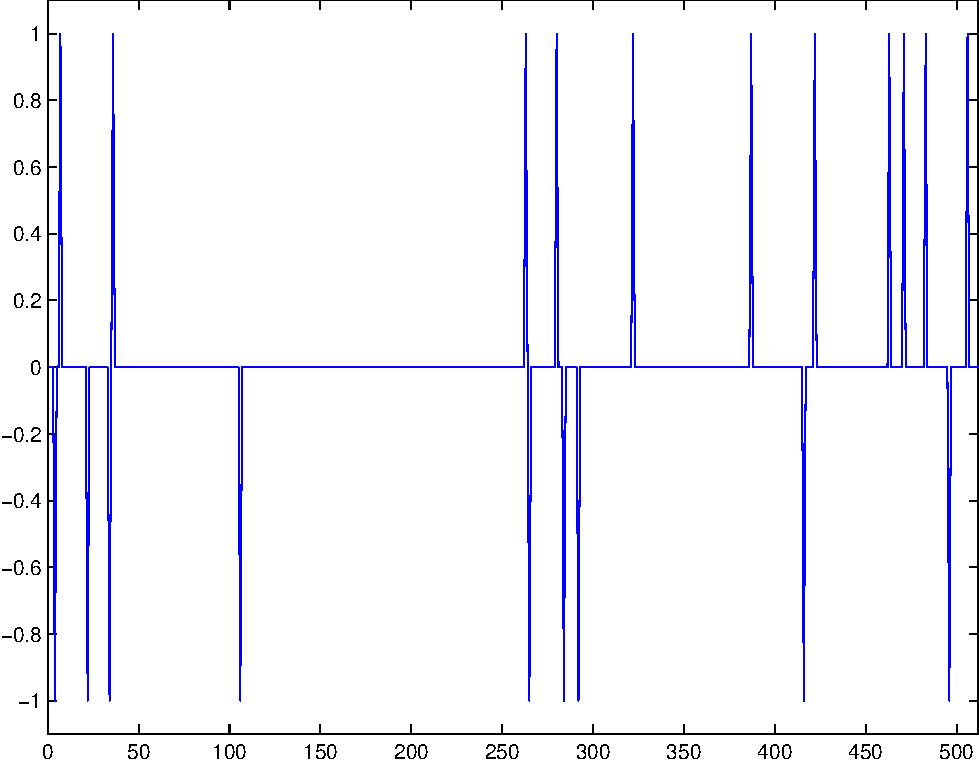
\includegraphics[height=1.5in]{Figs/l1eqexample_signal.pdf} & 
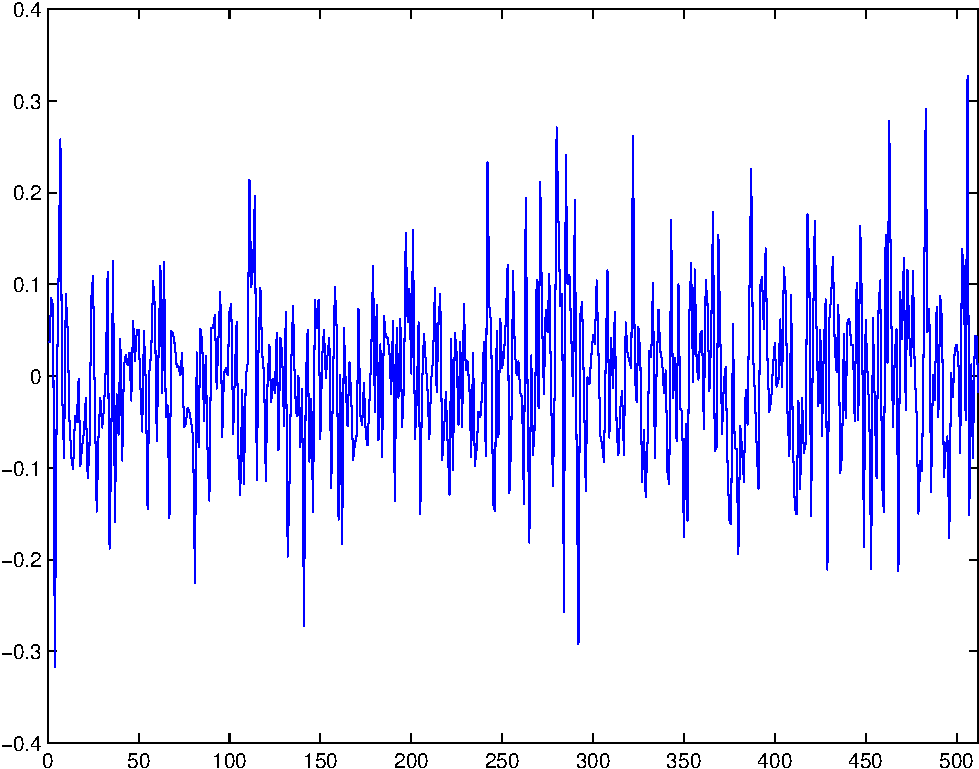
\includegraphics[height=1.5in]{Figs/l1eqexample_minl2.pdf}& 
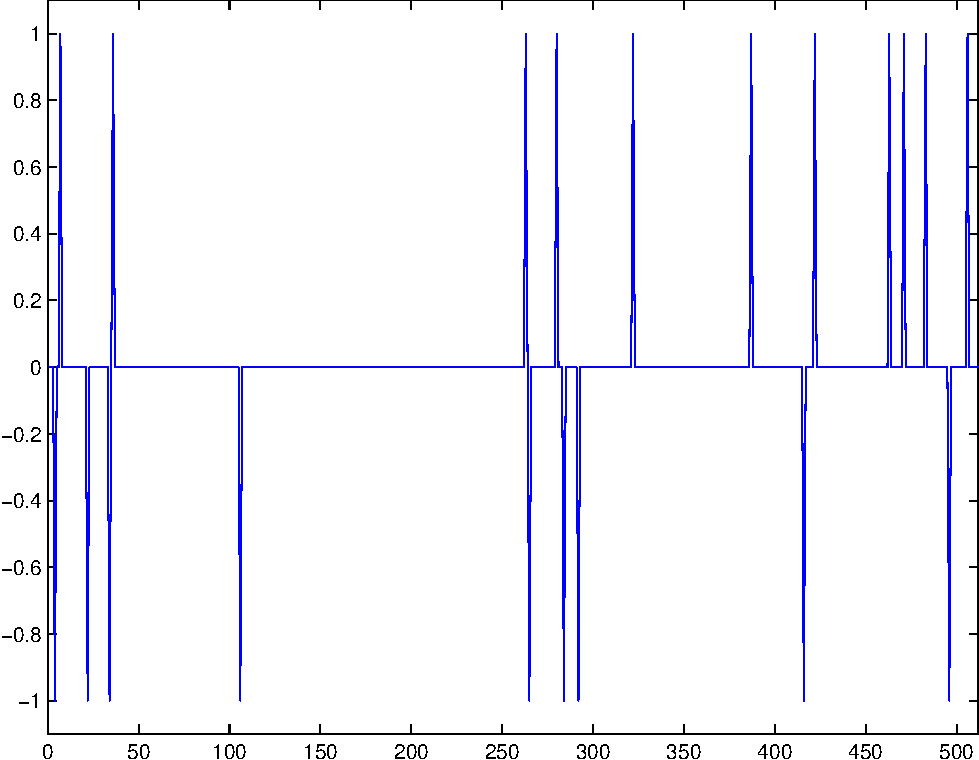
\includegraphics[height=1.5in]{Figs/l1eqexample_recovered.pdf} \\
(a) Original & (b) Minimum energy reconstruction & (c) Recovered
\end{tabular}
}
\caption{\small\sl 1D recovery experiment for $\ell_1$ minimization with equality constraints.  (a) Original length 512 signal \texttt{x} consisting of 20 spikes.  (b) Minimum energy (linear) reconstruction \texttt{x0}.  (c) Minimum $\ell_1$ reconstruction \texttt{xp}.}
\label{fig:l1eqexample}
\end{figure}
%%%


\subsection{Phantom reconstruction}

A large scale example is given in \texttt{tveq\_phantom\_example.m}.  This files recreates the phantom reconstruction experiment first published in \cite{candes04ro}.  The $256\times 256$ Shepp-Logan phantom, shown in Figure~\ref{fig:phantom}(a), is measured at $K=5481$ locations in the 2D Fourier plane; the sampling pattern is shown in Figure~\ref{fig:phantom}(b).  The image is then reconstructed exactly using $(TV_1)$.

The star-shaped Fourier-domain sampling pattern is created with
\begin{verbatim}
% number of radial lines in the Fourier domain
L = 22;

% Fourier samples we are given
[M,Mh,mh,mhi] = LineMask(L,n);
OMEGA = mhi;
\end{verbatim}
The auxiliary function \texttt{LineMask.m} (found in the `Measurements' subdirectory) creates the star-shaped pattern consisting of 22 lines through the origin.  The vector \texttt{OMEGA} 
contains the locations of the frequencies used in the sampling pattern.

This example differs from the previous one in that the code operates in {\em large-scale} mode.  The measurement matrix in this example is $5481\times 65536$, making the system \eqref{eq:lbnewton} far too large to solve (or even store) explicitly.  (In fact, the measurment matrix itself would require almost 3 gigabytes of memory if stored in double precision.)  Instead of creating the measurement matrix explicitly, we provide {\em function handles} that take a vector $x$, and return $Ax$.  As discussed above, the Newton steps are solved for using an implicit algorithm.

To create the implicit matrix, we use the function handles
\begin{verbatim}
A = @(z) A_fhp(z, OMEGA);
At = @(z) At_fhp(z, OMEGA, n);
\end{verbatim}
The function \texttt{A\_fhp.m} takes a length $N$ vector (we treat $n\times n$ images as $N:=n^2$ vectors), and returns samples on the $K$ frequencies.  (Actually, since the underlying image is real, \texttt{A\_fhp.m} return the real and imaginary parts of the 2D FFT on the upper half-plane of the domain shown in Figure~\ref{fig:phantom}(b).)  

To solve $(TV_1)$, we call
\begin{verbatim}
xp = tveq_logbarrier(xbp, A, At, y, 1e-1, 2, 1e-8, 600);
\end{verbatim}
The variable \texttt{xbp} is the initial guess (which is again the minimal energy reconstruction shown in Figure~\ref{fig:phantom}(c)), \texttt{y} are the measurements, and\texttt{1e-1} is the desired precision.  The sixth input is the value of $\mu$ (the amount by which to increase $\tau^k$ at each iteration; see Section~\ref{sec:logbarrier}).  The last two inputs are parameters for the large-scale solver used to find the Newton step.  The solvers are iterative, with each iteration requiring one application of \texttt{A} and one application of \texttt{At}.  The seventh and eighth arguments above state that we want the solver to iterate until the solution has precision $10^{-8}$ (that is, it finds a $z$ such that $\|Hz-g\|_2/\|g\|_2 \leq 10^{-8}$), or it has reached 600 iterations.

The recovered phantom is shown in Figure~\ref{fig:phantom}(d).  
We have $\|X_{TV}-X\|_2/\|X\|_2 \approx 8\cdot 10^{-3}$. 


%%%
\begin{figure}
\centerline{
\begin{tabular}{cccc}
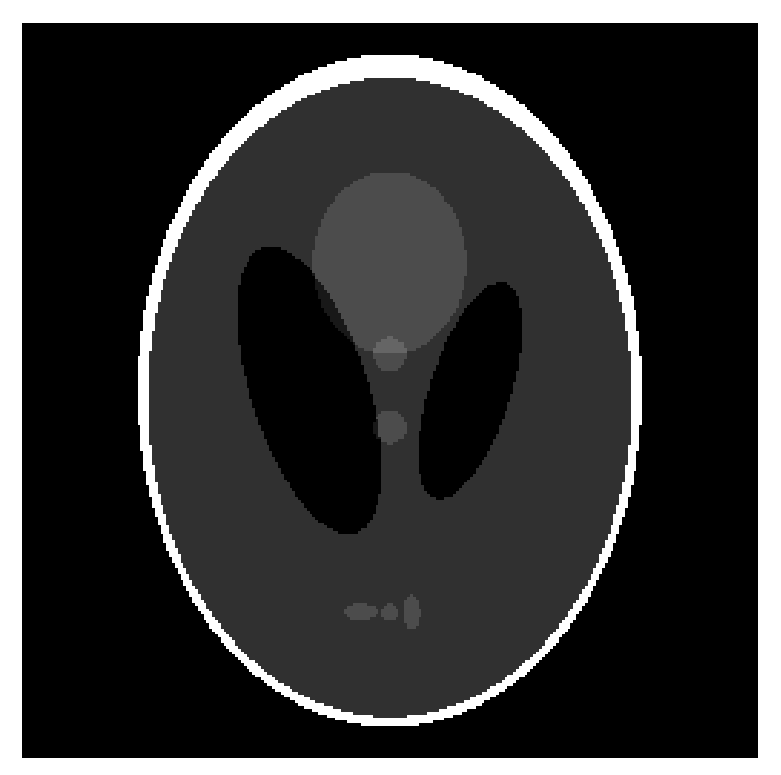
\includegraphics[height=1.5in]{Figs/phantom_orig} &
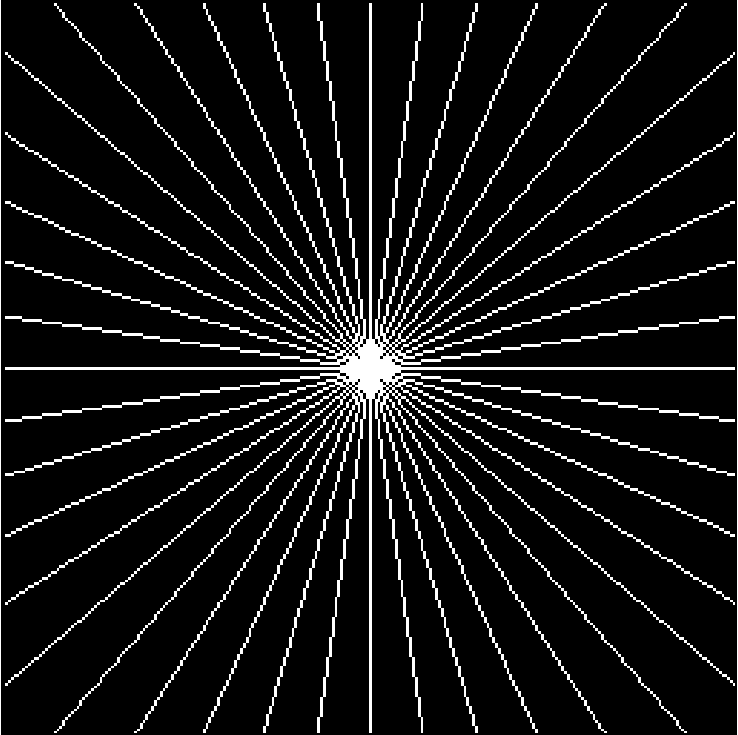
\includegraphics[height=1.5in]{Figs/phantom_sampling} &
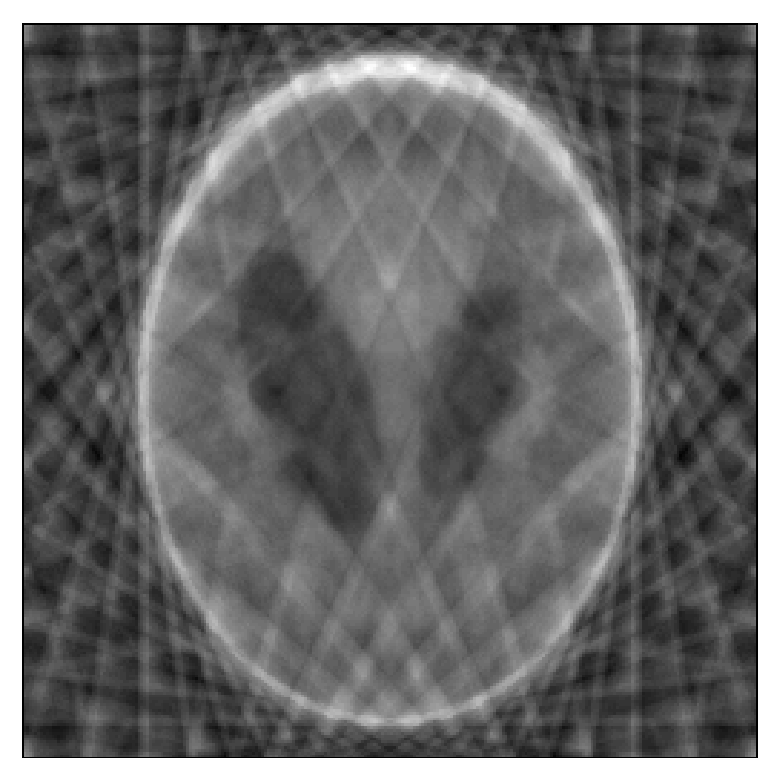
\includegraphics[height=1.5in]{Figs/phantom_backproj} &
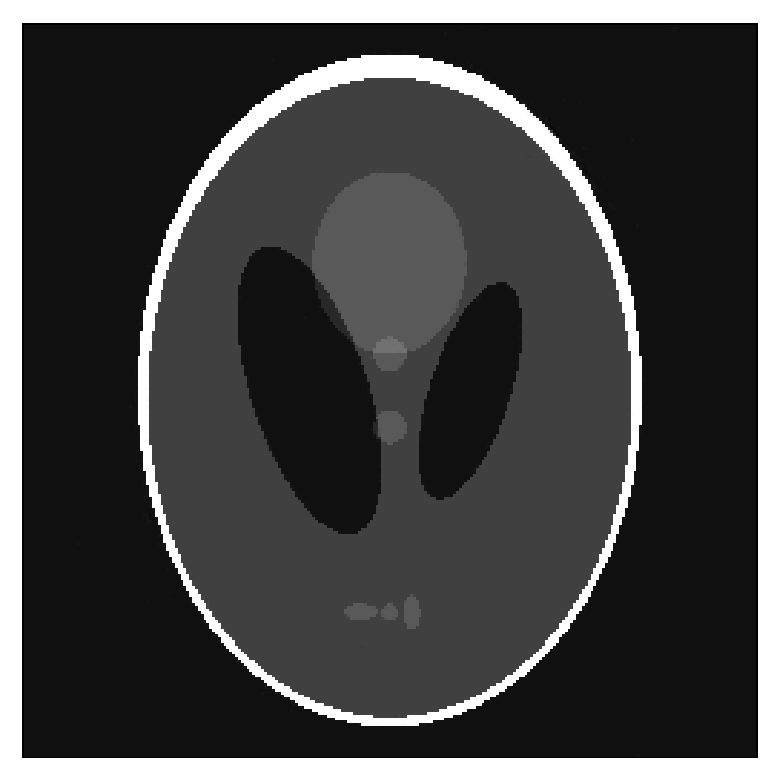
\includegraphics[height=1.5in]{Figs/phantom_tv} \\
{\small (a) Phantom} & {\small (b) Sampling pattern} &
{\small (c) Min energy} & {\small (d) min-TV reconstruction}
\end{tabular}
}
\caption{\small\sl Phantom recovery experiment.}
\label{fig:phantom}
\end{figure}
%%%

%-------------------------------------------------------------------------------
\subsection{Optimization routines}

We include a brief description of each of the main optimization routines (type
\texttt{help <function>} in MATLAB for details).  Each of these m-files is found in the \texttt{Optimization} subdirectory.

\begin{tabular}{|p{1.5 in}m{4 in}|} \hline
%
\texttt{cgsolve} & Solves $Ax=b$, where $A$ is symmetric positive definite, using the Conjugate Gradient method. \\[2mm]\hline
%
\texttt{l1dantzig\_pd} & Solves $(P_D)$ (the Dantzig selector) using a primal-dual algorithm. \\[2mm]\hline
%
\texttt{l1decode\_pd} & Solves the norm approximation problem $(P_A)$ (for decoding via linear programming) using a primal-dual algorithm. \\[2mm]\hline
%
\texttt{l1eq\_pd} & Solves the standard Basis Pursuit problem $(P_1)$ using a primal-dual algorithm.  \\[2mm]\hline
%
\texttt{l1qc\_logbarrier} & Barrier (``outer'') iterations for solving quadratically constrained $\ell_1$ minimization $(P_2)$. \\[2mm]\hline
%
\texttt {l1qc\_newton} & Newton (``inner'') iterations for solving quadratically constrained $\ell_1$ minimization $(P_2)$. \\[2mm]\hline
%
\texttt{tvdantzig\_logbarrier} & Barrier iterations for solving the TV Dantzig selector $(TV_D)$. \\[2mm]\hline
%
\texttt{tvdantzig\_newton} & Newton iterations for $(TV_D)$. \\[2mm]\hline
%
\texttt{tveq\_logbarrier} & Barrier iterations for equality constrained TV minimizaiton $(TV_1)$. \\[2mm]\hline
%
\texttt{tveq\_newton} & Newton iterations for $(TV_1)$. \\[2mm]\hline
%
\texttt{tvqc\_logbarrier} & Barrier iterations for quadratically constrained TV minimization $(TV_2)$. \\[2mm]\hline
%
\texttt{tvqc\_newton} & Newton iterations for $(TV_2)$. \\[2mm]\hline
%

\end{tabular}

%-------------------------------------------------------------------------------
\section{Error messages}

Here we briefly discuss each of the error messages that the $\ell_1$-{\sc magic} may produce.

\begin{itemize}
%
\item \texttt{Matrix ill-conditioned.  Returning previous iterate.}  
This error can occur when the code is running in {\em small-scale} mode; that is, the matrix $A$ is provided explicitly.  The error message is produced when the condition number of the 
linear system we need to solve to find the step direction (i.e.\ \eqref{eq:pdnewton} for the linear programs, and \eqref{eq:lbnewton} for the SOCPs) has an estimated condition number of less than $10^{-14}$.  

This error most commonly occurs during the last iterations of the primal-dual or log-barrier algorithms.  While it means that the solution is not within the tolerance specified (by the primal-dual gap), in practice it is usually pretty close.
%
\item  \texttt{Cannot solve system.  Returning previous iterate.}
This error is the large-scale analog to the above.  The error message is produced when the residual produced by the conjugate gradients algorithm was above $1/2$; essentially this means that CG has not solved the system in any meaningful way.  Again, this error typically occurs in the late stages of the optimization algorithm, and is a symptom of the system being ill-conditioned.
%
\item \texttt{Stuck backtracking, returning last iterate.}
This error occurs when the algorithm, after computing the step direction, cannot find a step size small enough that decreases the objective.  It is generally occurs in large-scale mode, and is a symptom of CG not solving for the step direction to sufficient precision (if the system is solved perfectly, a small enough step size will always be found).  Again, this will typically occur in the late stages of the optimization algorithm.
%
\item \texttt{Starting point infeasible; using x0 = At*inv(AAt)*y.}
Each of the optimization programs expects an initial guess which is {\em feasible} (obeys the constraints).  If the \texttt{x0} provided is not, this message is produced, and the algorithm proceeds using the least-squares starting point $x_0 = A^T(AA^T)^{-1}b$.
%
\end{itemize}

%-------------------------------------------------------------------------------

\newpage
\section*{Appendix}
\appendix

%-------------------------------------------------------------------------------
\section{$\ell_1$ minimization with equality constraints}

When $x$, $A$ and $b$ are real, then $(P_1)$ can be recast as the linear program
\begin{align*}
\min_{x,u}~\sum_i u_i \quad\text{subject~to}\quad
 x_i - u_i  & \leq 0 \\[-4mm]
 -x_i - u_i & \leq 0, \\
 Ax & = b
\end{align*}
which can be solved using the standard primal-dual algorithm outlined in Section~\ref{sec:primaldual}
(again, see \cite[Chap.11]{boyd04co} for a full discussion).
Set
\begin{eqnarray*}
f_{u_1;i} & := & x_i - u_i \\
f_{u_2;i} & := & -x_i - u_i,
\end{eqnarray*}
with $\lambda_{u_1;i},\lambda_{u_2;i}$ the corresponding dual variables, 
and let $f_{u_1}$ be the vector $(f_{u_1;1}~~\ldots~~f_{u_1;N})^T$ (and likewise for $f_{u_2},\lambda_{u_1},\lambda_{u_2}$).
Note that
\[
\grad f_{u_1;i} = \bpm \delta_i \\ -\delta_i \epm,
\quad
\grad f_{u_2;i} = \bpm -\delta_i \\ -\delta_i \epm,
\quad
\grad^2 f_{u_1;i} = 0,
\quad
\grad^2 f_{u_2;i} = 0,
\]
where $\delta_i$ is the standard basis vector for component $i$.  
Thus at a point $(x,u; v,\lambda_{u_1},\lambda_{u_2})$, the central and dual 
residuals are 
\begin{eqnarray*}
r_{\mathrm{cent}} & = & \bpm -\Lambda_{u_1} f_{u_1} \\ -\Lambda_{u_2} f_{u_2} \epm 
- (1/\tau)\mathbf{1}, \\
r_{\mathrm{dual}} & = & \bpm \lambda_{u_1}-\lambda_{u_2} + A^Tv \\ 
\mathbf{1} - \lambda_{u_1}-\lambda_{u_2} \epm,
\end{eqnarray*}
and the Newton step 
\eqref{eq:pdnewton} is given by:
\[
\bpm \Sigma_1 & \Sigma_2 & A^T \\ \Sigma_2 & \Sigma_1 & 0 \\ A & 0 & 0 \epm
\bpm \dx \\ \du \\ \dv \epm =
\bpm w_1 \\ w_2 \\ w_3 \epm :=
\bpm (-1/\tau)\cdot(-f^{-1}_{u_1} + f^{-1}_{u_2}) - A^Tv \\
-\mathbf{1} - (1/\tau)\cdot(f^{-1}_{u_1} + f^{-1}_{u_2}) \\
b - Ax \epm,
\]
with
\[
\Sigma_1 = \Lambda_{u_1} F^{-1}_{u_1} - \Lambda_{u_2} F^{-1}_{u_2}, \quad
\Sigma_2 = \Lambda_{u_1} F^{-1}_{u_1} + \Lambda_{u_2} F^{-1}_{u_2},
\]
(The $F_\bullet$, for example, are diagonal matrices with $(F_\bullet)_{ii} = f_{\bullet;i}$, and $f^{-1}_{\bullet;i} = 1/f_{\bullet;i}$.)
Setting
\[
\Sigma_x = \Sigma_1 - \Sigma_2^2\Sigma_1^{-1},
\]
we can eliminate 
\begin{eqnarray*}
\dx & = & \Sigma_x^{-1}(w_1 - \Sigma_2\Sigma_1^{-1}w_2 - A^T\dv)\\
\du & = & \Sigma_1^{-1}(w_2 - \Sigma_2\dx),
\end{eqnarray*}
and solve
\[
-A\Sigma_x^{-1}A^T\dv =  w_3 - A(\Sigma_x^{-1}w_1 - \Sigma_x^{-1}\Sigma_2\Sigma_1^{-1}w_2).
\]
This is a $K\times K$ positive definite system of equations, and can be solved using conjugate gradients.

Given $\dx,\du,\dv$, we calculate the change in the inequality dual variables as in \eqref{eq:dlambda}:
\begin{eqnarray*}
\dlam_{u_1}  & = & \Lambda_{u_1} F^{-1}_{u_1}(-\dx + \du) - \lambda_{u_1}  - (1/\tau)f^{-1}_{u_1} \\
\dlam_{u_2} & = & \Lambda_{u_2} F^{-1}_{u_2}(\dx+\du) - \lambda_{u_2} - (1/\tau)f^{-1}_{u_2}. 
\end{eqnarray*}

%The line search proceeds exactly as described in Section~\ref{sec:primaldual}.

%-------------------------------------------------------------------------------
\section{$\ell_1$ norm approximation}
\label{sec:l1approx}

The $\ell_1$ norm approximation problem $(P_A)$ can also be recast as a linear program:
\begin{align*}
\min_{x,u}~\sum_{m=1}^M u_m \quad\text{subject~to}\quad
 Ax - u -y & \leq 0 \\[-4mm]
 -Ax - u + y & \leq 0,
\end{align*}
(recall that unlike the other 6 problems, here the $M\times N$ matrix $A$ has more rows than columns).
For the primal-dual algorithm, we define
\[
f_{u_1} = A x - u - y,\quad
f_{u_2} = -A x - u + y.
\]
Given a vector of weights $\sigma\in\R^M$,
\[
\sum_m \sigma_m\grad f_{u_1;m} = 
\bpm A^T\sigma \\ -\sigma \epm, \quad
\sum_m \sigma_m\grad f_{u_2;m} = 
\bpm -A^T\sigma \\ -\sigma \epm,
\]
\[
\sum_m \sigma_m\grad f_{u_1;m}\grad f_{u_1;m}^T = 
\bpm A^T\Sigma A & -A^T\Sigma \\ -\Sigma A & \Sigma \epm,\quad
\sum_m \sigma_m\grad f_{u_2;m}\grad f_{u_2;m}^T = 
\bpm A^T\Sigma A & A^T\Sigma \\ \Sigma A & \Sigma \epm.
\]
At a point $(x,u;\lambda_{u_1},\lambda_{u_2})$, the dual residual is
\[
r_{\mathrm{dual}} = 
\bpm A^T(\lambda_{u_1}-\lambda_{u_2}) \\ -\lambda_{u_1}-\lambda_{u_2} \epm, 
\]
and the Newton step is the solution to
\[
\bpm A^T\Sigma_{11}A & A^T\Sigma_{12} \\ \Sigma_{12}A &  \Sigma_{11}\epm 
\bpm \dx \\ \du \epm = 
\bpm -(1/\tau)\cdot A^T(-f^{-1}_{u_1} + f^{-1}_{u_2}) \\ 
-\mathbf{1} - (1/\tau)\cdot(f^{-1}_{u_1} + f^{-1}_{u_2}) \epm :=
\bpm w_1 \\ w_2 \epm
\]
where
\begin{eqnarray*}
\Sigma_{11} & = & -\Lambda_{u_1} F^{-1}_{u_1} - \Lambda_{u_2} F^{-1}_{u_2} \\
\Sigma_{12} & = & \Lambda_{u_1} F^{-1}_{u_1} - \Lambda_{u_2} F^{-1}_{u_2}.
\end{eqnarray*}
Setting
\[
\Sigma_x = \Sigma_{11} - \Sigma^2_{12}\Sigma^{-1}_{11},
\]
we can eliminate $\du = \Sigma_{11}^{-1}(w_2 - \Sigma_{22}A\dx)$, and solve
\[
A^T\Sigma_x A\dx = w_1 - A^T\Sigma_{22}\Sigma^{-1}_{11}w_2
\]
for $\dx$.  Again, $A^T\Sigma_x A$ is a $N\times N$ symmetric positive definite matrix (it is straightforward to verify that each element on the diagonal of $\Sigma_x$ will be strictly positive), 
and so the Conjugate Gradients algorithm can be used for large-scale problems. 

Given $\dx,\du$, the step directions for the inequality dual variables are given by
\begin{eqnarray*}
\dlam_{u_1} & = & 
-\Lambda_{u_1} F^{-1}_{u_1} (A\dx-\du) - \lambda_{u_1} - (1/\tau)f^{-1}_{u_1} \\
\dlam_{u_2} & = & 
\Lambda_{u_2} F^{-1}_{u_2}(A\dx+\du) - \lambda_{u_2} - (1/\tau)f^{-1}_{u_2}.
\end{eqnarray*}

%-------------------------------------------------------------------------------
\section{$\ell_1$ Dantzig selection}
\label{sec:l1dantzig}

An equivalent linear program to $(P_D)$ in the real case is given by:
\begin{align*}
\min_{x,u}~\sum_i u_i \quad\text{subject~to}\quad
 x - u & \leq 0, \\[-4mm]
 -x - u & \leq 0, \\
 A^T r - \epsilon & \leq 0, \\
 -A^T r - \epsilon & \leq 0,
\end{align*}
where $r = Ax-b$.  Taking
\[
f_{u_1} = x - u,\quad
f_{u_2} = -x -u,\quad
f_{\epsilon_1} = A^T r - \epsilon,\quad
f_{\epsilon_2} = -A^T r - \epsilon,
\]
the residuals at a point 
$(x,u;\lambda_{u_1},\lambda_{u_2},\lambda_{\epsilon_1},\lambda_{\epsilon_2})$, 
the dual residual is
\[
r_{\mathrm{dual}} = 
\bpm \lambda_{u_1}-\lambda_{u_2} + A^TA(\lambda_{\epsilon_1} - \lambda_{\epsilon_2})
\\ \mathbf{1} - \lambda_{u_1}-\lambda_{u_2}\epm, 
\]
and the Newton step is the solution to
\[
\bpm A^TA\Sigma_{a}A^TA + \Sigma_{11} & \Sigma_{12} \\ 
\Sigma_{12} &  \Sigma_{11}\epm 
\bpm \dx \\ \du \epm = 
\bpm -(1/\tau)\cdot (A^TA(-f^{-1}_{\epsilon_1} + f^{-1}_{\epsilon_2})) -
f^{-1}_{u_1} + f^{-1}_{u_2} \\ 
-\mathbf{1} - (1/\tau)\cdot(f^{-1}_{u_1} + f^{-1}_{u_2}) \epm :=
\bpm w_1 \\ w_2 \epm
\]
where
\begin{eqnarray*}
\Sigma_{11} & = & -\Lambda_{u_1}F^{-1}_{u_1} - \Lambda_{u_2}F^{-1}_{u_2} \\
\Sigma_{12} & = &  \Lambda_{u_1}F^{-1}_{u_1} - \Lambda_{u_2}F^{-1}_{u_2} \\
\Sigma_a & = & -\Lambda_{\epsilon_1}F^{-1}_{\epsilon_1} - \Lambda_{\epsilon_2}F^{-1}_{\epsilon_2}.
\end{eqnarray*}
Again setting
\[
\Sigma_x = \Sigma_{11} - \Sigma^2_{12}\Sigma^{-1}_{11},
\]
we can eliminate
\[
\du = \Sigma^{-1}_{11}(w_2 - \Sigma_{12}\dx),
\]
and solve
\[
(A^TA\Sigma_a A^TA + \Sigma_x)\dx = w_1 - \Sigma_{12}\Sigma^{-1}_{11}w_2
\]
for $\dx$.  As before, the system is symmetric positive definite, and the CG algorithm can be used to solve it.

Given $\dx,\du$, the step directions for the inequality dual variables are given by
\begin{eqnarray*}
\dlam_{u_1} & = & -\Lambda_{u_1} F^{-1}_{u_1}(\dx-\du) - \lambda_{u_1} - (1/\tau)f^{-1}_{u_1} \\
\dlam_{u_2} & = & -\Lambda_{u_2} F^{-1}_{u_2}(-\dx-\du) - \lambda_{u_2} - (1/\tau)f^{-1}_{u_2} \\
\dlam_{\epsilon_1} & = & -\Lambda_{\epsilon_1} F^{-1}_{\epsilon_1}(A^TA\dx) - 
\lambda_{\epsilon_1} - (1/\tau)f^{-1}_{\epsilon_1} \\
\dlam_{\epsilon_2} & = &  -\Lambda_{\epsilon_2} F^{-1}_{\epsilon_2}(-A^TA\dx) - 
\lambda_{\epsilon_2} - (1/\tau)f^{-1}_{\epsilon_2}.
\end{eqnarray*} 



%-------------------------------------------------------------------------------
\section{$\ell_1$ minimization with quadratic constraints}
\label{sec:l1qc}

The quadractically constrained $\ell_1$ minimization problem $(P_2)$ can be recast as the second-order cone program
\begin{align*}
\min_{x,u}~\sum_i u_i \quad\text{subject~to}\quad
 x - u & \leq 0, \\[-4mm]
 -x - u & \leq 0, \\
 \frac{1}{2}\left(\|Ax-b\|^2_2 - \epsilon^2\right) & \leq 0.
\end{align*}
Taking
\[
f_{u_1} = x - u,\quad
f_{u_2} = -x -u,\quad
f_\epsilon = \frac{1}{2}\left(\|Ax-b\|^2_2 - \epsilon^2\right),
\]
we can write the Newton step (as in \eqref{eq:lbnewton}) at a point $(x,u)$ for a given $\tau$ as
\[
\bpm \Sigma_{11} - f_\epsilon^{-1}A^TA + f_\epsilon^{-2}A^Trr^TA & \Sigma_{12} \\
\Sigma_{12} & \Sigma_{11} \epm
\bpm \dx \\ \du \epm = 
\bpm
f_{u_1}^{-1} - f_{u_2}^{-1} + f_\epsilon^{-1}A^Tr \\
-\tau\mathbf{1} - f_{u_1}^{-1} - f_{u_2}^{-1}
\epm :=
\bpm w_1 \\ w_2 \epm
\]
where $r = Ax-b$, and
\begin{eqnarray*}
\Sigma_{11} & = & F_{u_1}^{-2} + F_{u_2}^{-2} \\
\Sigma_{12} & = & -F_{u_1}^{-2} + F_{u_2}^{-2}.
\end{eqnarray*}
As before, we set
\[
\Sigma_x = \Sigma_{11} - \Sigma_{12}^2\Sigma_{11}^{-1}
\]
and eliminate $\du$
\[
\du = \Sigma_{11}^{-1}(w_2 - \Sigma_{12}\dx),
\]
leaving us with the reduced system
\[
(\Sigma_x - f_\epsilon^{-1}A^TA + f_\epsilon^{-2}A^Trr^TA)\dx = 
w_1 - \Sigma_{12}\Sigma_{11}^{-1}w_2
\]
which is symmetric positive definite and can be solved using CG.  

%-------------------------------------------------------------------------------
\section{Total variation minimization with equality constraints}
\label{sec:tveq}

The equality constrained TV minimization problem
\[
\min_{x}~\operatorname{TV}(x)\quad\text{subject~to}\quad Ax=b,
\]
can be rewritten as the SOCP
\begin{align*}
\min_{t,x}~\sum_{ij} t_{ij} \quad\text{s.t.}\quad \|D_{ij}x\|_2 & \leq t_{ij} \\[-2mm]
 Ax &= b. 
\end{align*}
Defining the inequality functions
\begin{equation}
\label{eq:ftij}
f_{t_{ij}} = \frac{1}{2}\left(\|D_{ij}\|_2^2 - t^2_{ij}\right)\quad i,j=1,\ldots,n
\end{equation}
we have 
\[
\grad f_{t_{ij}} =
\left( \begin{array}{c} D^T_{ij}D_{ij} x \\ -t_{ij}\delta_{ij} \end{array}\right)
\]
\[
\grad f_{t_{ij}} \grad f_{t_{ij}}^T =
\bpm D^T_{ij}D_{ij} xx^TD^T_{ij}D_{ij} & 
-t_{ij}D^T_{ij}D_{ij}x\delta_{ij}^T \\
-t_{ij}\delta_{ij}x^T D^T_{ij}D_{ij} & 
t_{ij}^2\delta_{ij}\delta_{ij}^T \\
\epm,\quad
\grad^2 f_{t_{ij}} = 
\bpm D_{ij}^*D_{ij} & \vzero \\
\vzero & -\delta_{ij}\delta_{ij}^T 
\epm,
\]
where $\delta_{ij}$ is the Kronecker vector that is $1$ in entry $ij$ and zero elsewhere.
For future reference:
\[
\sum_{ij}\sigma_{ij} \grad f_{t_{ij}} = 
\bpm D_h^T\Sigma D_h x + D_v^T\Sigma D_v x \\ -\sigma t\epm,
\]
\[
\sum_{ij} \sigma_{ij} \grad f_{t_{ij}} \grad f_{t_{ij}}^T = 
\left(\begin{array}{cc}
B\Sigma B^T & -BT\Sigma  \\ -\Sigma TB^T & \Sigma T^2 
\end{array}\right),
\]
\[
\sum_{ij} \sigma_{ij} \grad^2 f_{t_{ij}} = 
\left(\begin{array}{cc}
D_h^T \Sigma D_h + D_v^T \Sigma D_v & \vzero \\ \vzero & -\Sigma
\end{array}\right)
\]
where $\Sigma = \diag(\{\sigma_{ij}\})$, $T = \diag(t)$, $D_h$ has the $D_{h;ij}$ as rows (and likewise for $D_v$), and  $B$ is a matrix that depends on $x$:
\[
B = D_h^T\Sigma_{\partial h} + D_v^T\Sigma_{\partial v}.
\]
with $\Sigma_{\partial h} = \diag(D_h x),~ \Sigma_{\partial v} = \diag(D_v x)$.


The Newton system \eqref{eq:lbnewton} for the log-barrier algorithm is then
\[
\bpm H_{11} & B\Sigma_{12} & A^T \\ 
\Sigma_{12}B^T & \Sigma_{22} & \vzero \\
A & \vzero & \vzero \epm
\bpm \dx \\ \dt \\ \dv \epm ~=~
\bpm  D_h^T F_t^{-1} D_h x + D_v^T F_t^{-1} D_vx \\ 
-\tau\mathbf{1} - F_{t}^{-1}t \\ 
\vzero \epm ~:= ~
\bpm w_1 \\ w_2 \\ \vzero \epm,
\]
where 
\[
H_{11} = D_h^T(-F_t^{-1})D_h ~+~ D_v^T(-F_t^{-1})D_v ~+~ B F_t^{-2}B^T.
\]
Eliminating $\dt$
\begin{eqnarray*}
\dt & = & \Sigma_{22}^{-1}(w_2 - \Sigma_{12}B^T\dx) \\
 & = & \Sigma_{22}^{-1}(w_2 - \Sigma_{12}\Sigma_{\partial h}D_h\dx - \Sigma_{12}\Sigma_{\partial v}D_v\dx),
\end{eqnarray*}
the reduced $(N+K)\times (N+K)$ system is
\begin{equation}
\label{eq:tveqsys}
\bpm H'_{11} & A^T \\ A & \vzero \epm
\bpm \dx \\ \dv \epm = 
\bpm w'_1 \\ \vzero \epm
\end{equation}
with
\begin{align*}
H'_{11} = ~& H_{11} - B\Sigma^2_{12}\Sigma_{22}^{-1}B^T \\
= ~& D_h^T(\Sigma_b\Sigma^2_{\partial h}-F_t^{-1})D_h ~+~
D_v^T(\Sigma_b\Sigma^2_{\partial v}-F_t^{-1})D_v ~+~\\
~& D_h^T(\Sigma_b\Sigma_{\partial h}\Sigma_{\partial v})D_v ~+~
D_v^T(\Sigma_b\Sigma_{\partial h}\Sigma_{\partial v})D_h\\
w'_1 = ~& w_1 - B\Sigma_{12}\Sigma_{22}^{-1}w_2 \\
 = ~& w_1 - (D_h^T\Sigma_{\partial h} + D_v^T\Sigma_{\partial v} )\Sigma_{12}\Sigma_{22}^{-1}w_2 \\
\Sigma_b = ~& F_t^{-2} - \Sigma_{22}^{-1}\Sigma_{12}^2. 
\end{align*}

The system of equations \eqref{eq:tveqsys} is symmetric, but not positive definite.
Note that $D_h$ and $D_v$ are (very) sparse matrices, and hence can be stored and applied very efficiently.  This allows us to again solve the system above using an iterative method such as SYMMLQ \cite{paige75so}.



%-------------------------------------------------------------------------------
\section{Total variation minimization with quadratic constraints}
\label{sec:tvqc}

We can rewrite $(TV_2)$ as the SOCP
\begin{align*}
\min_{x,t}~\sum_{ij} t_{ij}
\quad\text{subject~to}\quad
& \|D_{ij} x\|_2\leq t_{ij}, ~~ i,j=1,\ldots,n \\[-4mm]
& \|Ax - b\|_2 \leq \epsilon
\end{align*}
where $D_{ij}$ is as in \eqref{eq:Dij}.
%
Taking $f_{t_{ij}}$ as in \eqref{eq:ftij} and 
\[
f_\epsilon = \frac{1}{2}\left( \|Ax-b\|^2_2 - \epsilon^2\right),
\]
with
\[
\grad f_\epsilon = \bpm A^Tr \\ \vzero \epm,\quad 
\grad f_\epsilon \grad f_\epsilon^T =
\bpm  A^Trr^TA & \vzero \\ \vzero & \vzero \epm, \quad
\grad^2 f_\epsilon = \bpm A^*A & \vzero \\
\vzero & \vzero \epm
\]
where $r = Ax-b$.


 Also,
\[
\grad^2 f_{t_{ij}} = \left(\begin{array}{cc} D_{ij}^*D_{ij} & \vzero \\
\vzero & -\delta_{ij}\delta_{ij}^T \end{array}\right)
\quad
\grad^2 f_\epsilon = \left(\begin{array}{cc} A^*A & \vzero \\
\vzero & \vzero \end{array}\right).
\]

The Newton system is similar to that in equality constraints case:
\[ 
\bpm H_{11} & B\Sigma_{12} \\
\Sigma_{12}B^T & \Sigma_{22} \epm
\bpm \dx \\ \dt \epm =
\bpm D_h^T F_t^{-1}D_h x + D_v^TF_t^{-1}D_v x + f_\epsilon^{-1}A^Tr \\
-\tau\mathbf{1} - tf^{-1}_t \epm :=
\bpm w_1 \\ w_2 \epm.
\]
where $(tf^{-1}_t)_{ij} = t_{ij}/f_{t_{ij}}$, and 
\begin{align*}
H_{11} = ~& D_h^T(-F_t^{-1})D_h ~+~ D_v^T(-F_t^{-1})D_v ~+~ B F_t^{-2}B^T ~- \\
 & f_\epsilon^{-1} A^TA ~+~ f_\epsilon^{-2} A^Trr^TA, \\
\Sigma_{12} = ~& -TF_t^{-2}, \\
\Sigma_{22} = ~& F_t^{-1} + F_t^{-2}T^2,
\end{align*}
Again eliminating $\dt$
\[
\dt = \Sigma_{22}^{-1}(w_2 - \Sigma_{12}\Sigma_{\partial h}D_h\dx - \Sigma_{12}\Sigma_{\partial v}D_v\dx),
\]
the key system is
\[
H'_{11}\dx  = 
w_1 - (D_h^T\Sigma_{\partial h} + D_v^T\Sigma_{\partial v} )\Sigma_{12}\Sigma_{22}^{-1}w_2
\]
where
\begin{align*}
H'_{11} = ~& H_{11} - B\Sigma^2_{12}\Sigma_{22}^{-1}B^T \\
= ~& D_h^T(\Sigma_b\Sigma^2_{\partial h}-F_t^{-1})D_h ~+~
D_v^T(\Sigma_b\Sigma^2_{\partial v}-F_t^{-1})D_v ~+~\\
~& D_h^T(\Sigma_b\Sigma_{\partial h}\Sigma_{\partial v})D_v ~+~
D_v^T(\Sigma_b\Sigma_{\partial h}\Sigma_{\partial v})D_h ~-~ \\
~& f_\epsilon^{-1} A^TA ~+~ f_\epsilon^{-2} A^Trr^TA, \\
\Sigma_b = ~& F_t^{-2} - \Sigma_{12}^2\Sigma_{22}^{-1}.
\end{align*}

The system above is symmetric positive definite, and can be solved with CG.


%-------------------------------------------------------------------------------
\section{Total variation minimization with bounded residual correlation}
\label{sec:tvdantzig}

The $TV$ Dantzig problem has an equivalent SOCP as well:
\begin{align*}
\min_{x,t}~\sum_{ij} t_{ij}
\quad\text{subject to}\quad\quad
\|D_{ij} x\|_2 & \leq t_{ij}, ~~ i,j=1,\ldots,n \\[-4mm]
A^T(Ax-b) -\epsilon & \leq 0 \\
-A^T(Ax-b) -\epsilon & \leq 0.
\end{align*}
%
The inequality constraint functions are
\begin{eqnarray*}
f_{t_{ij}} & = & \frac{1}{2}\left( \|D_{ij}x\|^2_2 - t_{ij}^2\right) \quad i,j=1,\ldots,n\\
f_{\epsilon_1} & = & A^T(Ax-b)-\epsilon, \\
f_{\epsilon_2} & = & -A^T(Ax-b)-\epsilon,
\end{eqnarray*}
with
\[
\sum_{ij}\sigma_{ij} \grad f_{\epsilon_1;ij} = 
\bpm A^TA\sigma \\ \vzero \epm, \quad
\sum_{ij}\sigma_{ij} \grad f_{\epsilon_2;ij} = 
\bpm -A^TA\sigma \\ \vzero \epm,
\]
and
\[
\sum_{ij} \sigma_{ij} \grad f_{\epsilon_1;ij} \grad f_{\epsilon_1;ij}^T = 
\sum_{ij} \sigma_{ij} \grad f_{\epsilon_2;ij} \grad f_{\epsilon_2;ij}^T =
\bpm A^TA\Sigma A^TA & \vzero \\ \vzero & \vzero \epm.
\]
Thus the log barrier Newton system is nearly the same as in the quadratically constrained case:
\[
\bpm H_{11} & B\Sigma_{12} \\
\Sigma_{12}B^T & \Sigma_{22} \epm
\bpm \dx \\ \dt \epm =
\bpm D_h^T F_t^{-1}D_h x + D_v^TF_t^{-1}D_v x + 
A^TA(f_{\epsilon_1}^{-1}-f_{\epsilon_2}^{-1}) \\
-\tau\mathbf{1} - tf^{-1}_t \epm :=
\bpm w_1 \\ w_2 \epm.
\]
where
\begin{align*}
H_{11} = ~& D_h^T(-F_t^{-1})D_h ~+~ D_v^T(-F_t^{-1})D_v ~+~ B F_t^{-2}B^T ~+~ A^TA\Sigma_a A^TA, \\
\Sigma_{12} = ~& -TF_t^{-2}, \\
\Sigma_{22} = ~& F_t^{-1} + F_t^{-2}T^2, \\
\Sigma_a = ~& F_{\epsilon_1}^{-2} + F_{\epsilon_2}^{-2}.
\end{align*}
Eliminating $\dt$ as before
\[
\dt ~=~ \Sigma_{22}^{-1}(w_2 - \Sigma_{12}\Sigma_{\partial h}D_h\dx - 
\Sigma_{12}\Sigma_{\partial v}D_v\dx),
\]
the key system is
\[
H'_{11}\dx  =  
w_1 - (D_h^T\Sigma_{\partial h} + D_v^T\Sigma_{\partial v} )\Sigma_{12}\Sigma_{22}^{-1}w_2
\]
where
\begin{align*}
H'_{11} = ~& D_h^T(\Sigma_b\Sigma^2_{\partial h}-F_t^{-1})D_h ~+~
D_v^T(\Sigma_b\Sigma^2_{\partial v}-F_t^{-1})D_v ~+~\\
~& D_h^T(\Sigma_b\Sigma_{\partial h}\Sigma_{\partial v})D_v ~+~
D_v^T(\Sigma_b\Sigma_{\partial h}\Sigma_{\partial v})D_h ~+~ 
A^TA\Sigma_a A^TA, \\
\Sigma_b = ~& F_t^{-2} - \Sigma_{12}^2\Sigma_{22}^{-1}.
\end{align*}






%-------------------------------------------------------------------------------
\vspace{10mm}

\bibliographystyle{plain}
\bibliography{l1magic}

\end{document}
